\chapter{Abstracted View of the System}
	\label{4}
	In this chapter, we will introduce the architecture of our system, explaining the essential elements
	that is composed of, and their interactions.
	\begin{figure}[H]
		\iftrue
		\caption{Essential System Components}
		\centering
		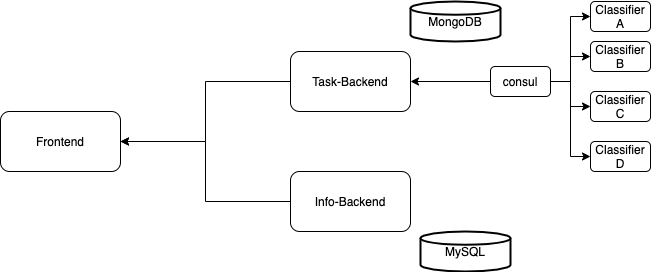
\includegraphics[scale=0.3]{figures/system-overview}
		\fi
	\end{figure}
	\section{Frontend Web App}
		The Frontend component has the responsibility of being the edge in our system.
		\begin{figure}[H]
			\iftrue
			\caption{Our system's edge}
			\centering
			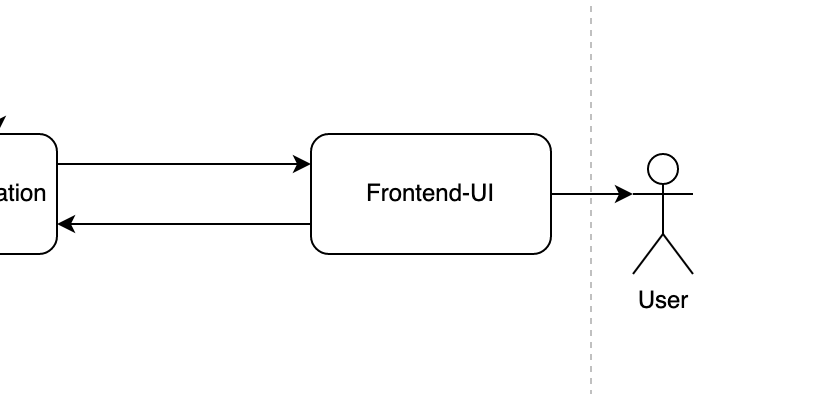
\includegraphics[scale=0.3]{figures/frontend-actor}
			\fi
		\end{figure}
		Every action from our users, should be channeled through the frontend.Our frontend is a web-based application, 
		and as an consequence of that, a design desision is that the API between the web app and the backend application
		will not be a public one. This desision will increase the security of our system, as the proccess of writing 
		spam bots will be significantly harder without a known API. More information about the API(Application 
		programming interface) will be given below.
	\section{Backend}
		There is a number of design choices that we have made on our Backend System, in order to increase security, and
		decrese complexity. Our Backend System follows the design principles of the microservice pattern. Microservice pattern
		tries to decrease complexity and increase safety by splitting the internal logic of a system into several components called
		'Microservices'. Each microservice is essentially a server that handles a small portion of the systems logic. As opposed to the
		monolithic services, microservices have a number of advantages such as
		\begin{itemize}
			\item Highly maintainable and testable
			\item Loosely coupled
			\item Independently deployable
			\item No Single Point of Failure
		\end{itemize}
		\subsection{Information Backend}
			The first of our services is the Information Backend. This service will have the responsibility to handle the information
			related to a scan, as well as its statistics and ascosiations between scans and patients. The majority of the models composing
			our systems will be available though this service, via a well designed API.
		\subsection{Task Backend}
			This microservice will have the responsibility to trigger prediction and classification tasks for our system. The whole procedure,
			due to its CPU Intensive nature, will have to be asyncronous and to be executed in the background. The Frontend will sent a request for
			a given task, and the server will have to return a token, ascosiated for that particular task. Later, The frontend may request to learn the
			progress of its task or its results(if completed) by using the relevant token. This design choice is unavoidable given that the HTTP protocol
			has embedded the notion of 'timeout', it is just impossible and impractical to wait untill a given task is complete. Another great advantage of 
			this asyncronous design is the fact that multiple users may request Tasks without eliminating the server's resources, such as CPU time and amount of
			RAM available. Indepedent of the number of requests, the server will implement a queue FIFO (First-In-First-Out) strategy and it will inform its users
			when the task is ready to be seen. 
		\subsection{Classification Backend}
			By using multiple classification techniques, our system will reduce the probability of an false prediction further. So one of our 
		
		
		
				
					
			
		
	
